\section{Reproducible computations and numerical behavior}
\label{sec:computations}

The analytic proof has three independently evaluable descriptions:
the convolution recurrence, the spectral measure of a positive operator,
and the endpoint Laplace integral. The supplied experiments compare
them. None of the numerical calculations is used as a substitute for
an infinite-dimensional argument or an asymptotic remainder proof.

\subsection{Precision and independent representations}

The principal run computes the recurrence through $n=1000$ using
370 decimal digits. It propagates $u_n=\rho^ng_n$ so that large
intermediate values are avoided, and then recovers
$E_n=\rho^{-n}(\gamma-u_n)$. Since this subtraction loses about
$n\log_{10}(1/\rho)$ digits, ordinary machine precision would be
unsuitable. A higher-precision comparison is included in the run log.

An independent calculation replaces the integral in $J$ by
Gauss--Legendre quadrature. This gives a finite symmetric matrix
with one central coordinate and diagonal entries at the quadrature
nodes. Its spectral weights approximate the continuous positive
measure. We used 128, 256, and 512 nodes. At the largest resolution,
the worst sampled relative discrepancy in the residual is about
$1.1\times10^{-8}$. This discretization evaluates the small residual
from positive spectral weights and does not subtract the dominant
exponential term.

A third calculation uses the exact local identity for $P(s)$ and
rescales the integral by $y=ns$. The recorded run uses 70 decimal
digits, a local series of degree 24, and a scaled cutoff of 120.
A sensitivity run uses 90 digits, degree 32, and cutoff 160.
For that stronger run, agreement with the recurrence has relative
discrepancy below $5\times10^{-44}$ at $n=50$ and below
$4\times10^{-66}$ at $n=256,1000$.
Those figures describe agreement between numerical calculations;
they are not directed-rounding error certificates.

The scripts also check the exact symbolic coefficient identities,
the Taylor coefficients of the algebraic expansion, and the finite
geometric identity underlying the product bounds. The stored
floating diagnostics record positive $E_n$ for all computed indices
and positive alternating differences at sampled orders through six.
Strict positivity for every index and order follows from the proof,
not from this finite sample.

\subsection{Why the leading asymptotic can be misleading at first}

\begin{table}[htbp]
\centering
\caption{Normalized residual from the scaled positive integral.
Values are floating diagnostics, rounded to ten decimal places.}
\label{tab:normalized}
\begin{tabular}{@{}rr@{}}
\toprule
$n$ & $n^2(\log n)^2E_n$\\
\midrule
\tableinput data/table_normalized.tex
\bottomrule
\end{tabular}
\end{table}

Table~\ref{tab:normalized} illustrates slow logarithmic convergence.
The normalized quantity passes through one and overshoots before
returning toward its limit. This is compatible with the eventual
positive first correction $2/\log n$. Complete monotonicity applies
to $E_n$, not to the separately normalized sequence
$n^2(\log n)^2E_n$.

\begin{figure}[htbp]
\centering
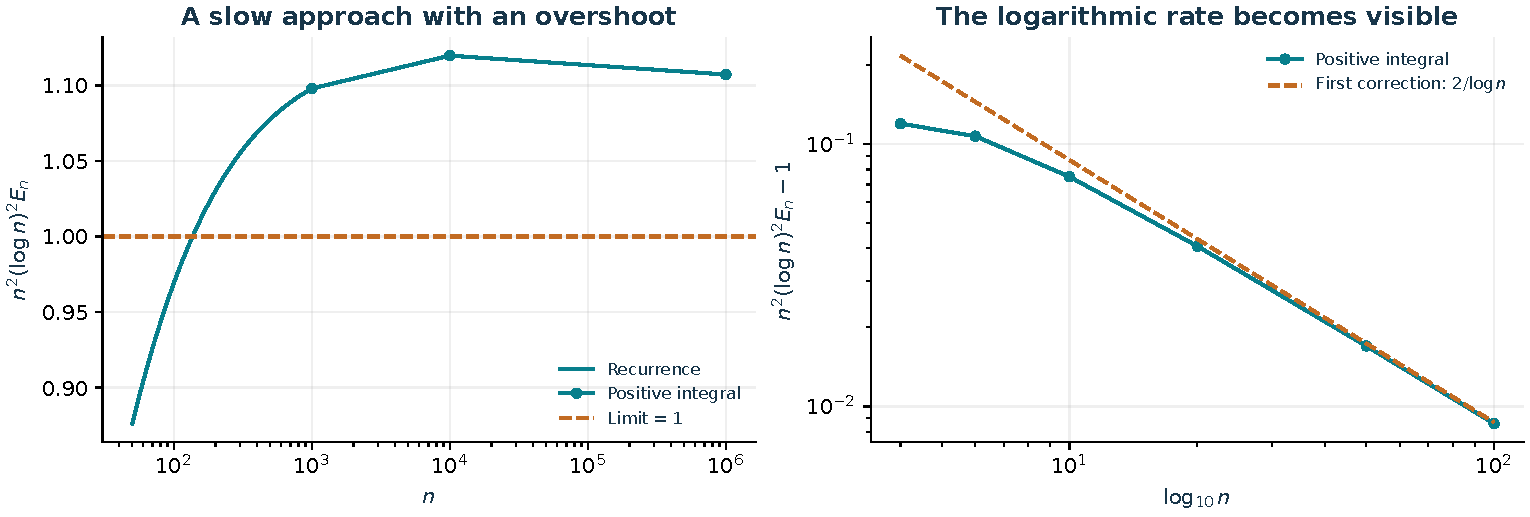
\includegraphics[width=\linewidth]{figures/normalized_remainder.pdf}
\caption{The finite-index approach and the eventual logarithmic rate.
The right horizontal axis is $\log_{10}n$, itself displayed on a
logarithmic scale. The curve $2/\log n$ is the first proved
relative correction, not a fitted model.}
\label{fig:normalized}
\end{figure}

Nor does a longer fixed inverse-logarithmic truncation always improve
a numerical approximation. For example, at $n=1000$, including
$c_0,\ldots,c_3$ gives relative error approximately
$-7.17\times10^{-4}$, whereas including $c_4$ as well gives
approximately $-1.67\times10^{-2}$. Asymptotic expansions assert
improvement as the limiting parameter tends to infinity at fixed
order, not a pointwise monotonic improvement with the order.

\subsection{Accuracy when the logarithmic integrals are retained}

Define the three successive approximations
\begin{align*}
 A_0(n)&=n^{-2}F_2(\log n),\\
 A_1(n)&=A_0(n)+(2n^3)^{-1}F_3(\log n),\\
 A_2(n)&=A_1(n)+n^{-4}
       \{F_4(\log n)/12-p_2F_4'(\log n)\}.
\end{align*}
Their errors, computed against the positive endpoint integral, are
shown in Table~\ref{tab:sectors}. The signs are retained in the table;
the plot uses absolute relative error. The next proved coefficient
in \eqref{eq:main-sectors} explains the remaining error of $A_2$.

\begin{table}[htbp]
\centering
\caption{Signed relative errors $A_j(n)/E_n-1$.}
\label{tab:sectors}
\begin{tabular}{@{}rrrr@{}}
\toprule
$n$ & $A_0$ & $A_1$ & $A_2$\\
\midrule
\tableinput data/table_sector_errors.tex
\bottomrule
\end{tabular}
\end{table}

\begin{figure}[htbp]
\centering
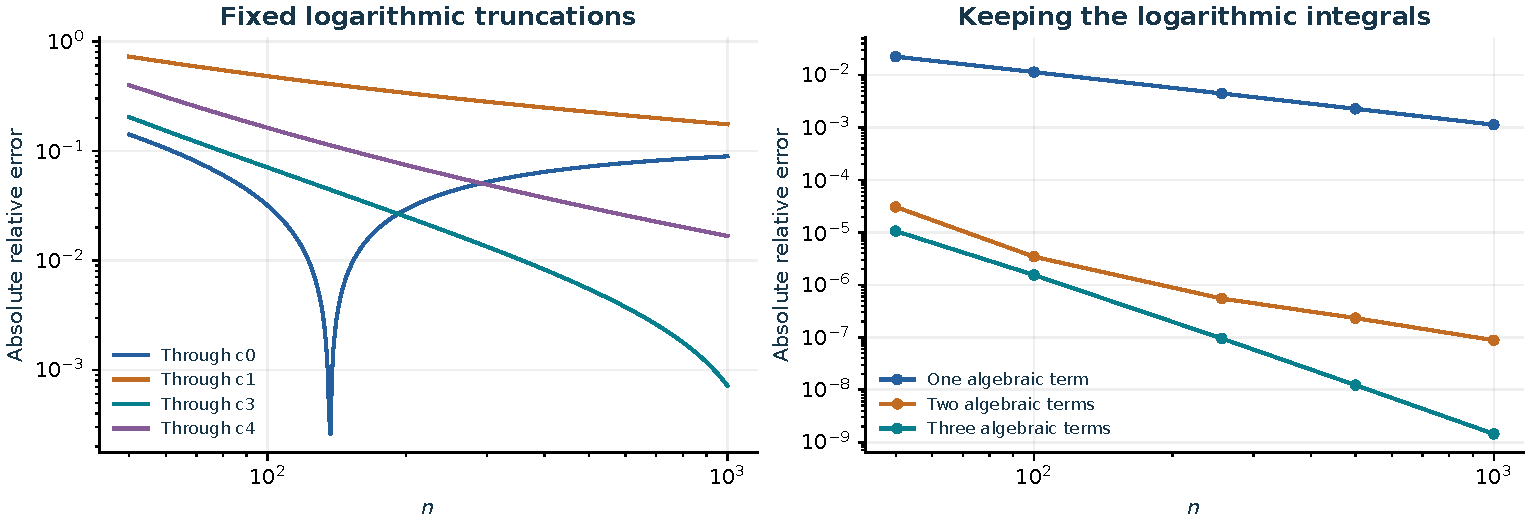
\includegraphics[width=\linewidth]{figures/approximation_errors.pdf}
\caption{Two types of approximation. On the left, a fixed number of
logarithmic terms may suffer cancellation or grow inaccurate at
moderate indices. On the right, the exact logarithmic integrals are
retained while successive powers of $1/n$ are added.}
\label{fig:errors}
\end{figure}

\subsection{The product constant}

The recorded finite product at $m=1000$ is
\[
 P_{1000}=0.61788133434828841381086077163828710263\ldots.
\]
The theorem proves that it lies above $C_*$, and
\eqref{eq:C-enclosure} provides an explicit tail enclosure in exact
arithmetic. The displayed decimal is a high-precision numerical
estimate of the finite product, rather than a certified decimal
enclosure of the infinite one.

\begin{table}[htbp]
\centering
\caption{Selected normalized partial products $P_m$, rounded by
truncating the displayed decimal expansion.}
\label{tab:product}
\begin{tabular}{@{}rl@{}}
\toprule
$m$ & $P_m$\\
\midrule
\tableinput data/table_product.tex
\bottomrule
\end{tabular}
\end{table}

\subsection{Reproduction commands and scope}

The Python programs require \texttt{mpmath}, \texttt{sympy},
\texttt{numpy}, \texttt{scipy}, and \texttt{matplotlib}. Versions
used in preparation are recorded in the data. From the package root:
\begin{verbatim}
python code/verify_recurrence.py --nmax 1000 --out rerun/data
python code/verify_symbolic.py --out rerun/symbolic_checks.json
python code/make_figures.py --input rerun/data --out rerun
make pdf
\end{verbatim}
The first three commands keep the originally supplied data intact.
Compilation uses the already included figures and tables, so building
the PDF does not require numerical libraries or network access.
Normal Python and optimized \texttt{python -O} runs produced the
same deterministic numerical data files in the preparation checks.
Runtime measurements and metadata are not expected to be identical
across machines.
